\chapter{Reduced Electronic Density Distribution} \label{ED}

A heterojuntion is basically a p-n junction in a semiconductor between
materials of different composition. Normal junctions are between p and n type
versions of the same material. But in this case we refer to a juntion formed
betewen two group III-arsenide usually a GaAs/AlAs interface or a GaAs/AlGaAs
interface. Since they are two differnt materials, the band structure is
discontinuous from one material to the other and the band alignment across the
interface is typically of type I, i.e. the band gap of the lower bandgap
material is positioned energetically within the bandgap of the wider bandgap
semiconductor.

Polarization fields 
The usual growth direction for hexagonal III-V materials is
along the polar [0001] axis, for which the crystal lacks inversion symeetry.
This will result in the formation of polarization fields. There are two kinds
of polarization fields. They are spontaneous polarization (SP) and
Piezoelectric polarization (PZ).  The spontaneous polarization exists in polar
semiconductors with a Wurzite or lower symmetry crystal structure and is
related to the deviation of the crystal lattice parameters from the ideal
values for the structure, thereby creating molecular dipoles in the material
building a polarization field just like that formed in ferroelectrics. This
field has a fixed direction along the [0001] c-axis in the Wurtzite lattice.
Therefore the field resulting from spontaneous polarization will point along
the growth direction and this maximizes pontaneous polarization effect in these
systems and renders the problem effectively one-dimensional.

The other type of polarization field, the piezoelectric polarization occurs due
to the presence of strain in the system. When two layers are joined together to
form a heterojunction, the difference in the lattice constant between the two
materials will lead to a strain . This strain also occurs due tot he difference
in the thermal expansion coefficients in the the layers during cool down after
growth. This leads to elastic strain in the layers. 

\section{Self-consistent Schr{\"o}dinger-Poisson Solver} \label{sec:model}

\subsection{Finite Element Method}\label{sec:FEM}

The study of energy band structures of heterostructures needs a detailed
knowledge of optical and transport properties of the heterostructures. These
properties can be found by solving self-consistently Poisson's and
Schr{\"o}dinger's equations for the electron wave functions.


The finite element method (FEM) is a simple and efficient method for solving
ordinary differential equations (ODEs) or partial differential equations (PDSs)
in problem regions with simple boundaries~\cite{bathe2006finite}. FEM can be used to solve for the
Schr{\"o}dinger and Poisson equation self-consistently. A generic formulation for a PDE with the following form: 

\begin{equation}
  |D|u(x) = f(x)\in\Omega
  \label{eq:generic}
\end{equation}

where $D$ is an arbitrary operator, and $\Omega$ defines the geometry. In order
to solve this PDE using FEM, eq.~\ref{eq:generic} has to be rewritten in weak
variational form with the boudary conditions:

\begin{eqnarray}
\begin{aligned}
  \left\{
    \begin{array}{ll} 
      u(x) = u_{0}(x) \qquad on \quad \Gamma_D   \\
      \frac{\partial{u}}{\partial{n}} = g_0(x) \qquad on \quad \Gamma_N
    \end{array}
  \right.
\end{aligned}
\label{eq:generic_BC}
\end{eqnarray}

where $\Gamma_D$ and $\Gamma_N$ signifies Dirichlet and Neumann boundary
condition. By introducing an arbitrary function $v$ and multiplying the PDF
with $v$, then integrating over all the domain $\Gamma$ and separating every
second-order derivative using integration by parts, the original PDE can be
carried out in the weak form as:

\begin{equation}
  \int_{\Omega}|D^\prime|(u{\cdot}v)\ d\Omega + \\
  \int_{\Gamma_N}gv\ \partial\Omega = \\
  \int_{\Omega}fv\ d\Omega \quad \forall v \in \hat{V}\\
  \label{eq:weakPDE}
\end{equation}

where $D^\prime$ is the reduced operator after performing integration by part to the second-order derivatives, and $\hat{V}$ is the function space where an arbitrary function $v$ belongs to. The function $u$ lies in V, which could be different than $\hat{V}$. This continuous variational problem need to be reformulated to discrete problem with discrete space $\hat{V}_d \subset \hat{V}$ and $V\subset{V}$ so that the boundary conditions can be restated as:

\begin{equation}
  \int_{\Omega}|D^\prime|(u_d{\cdot}v)\ d\Omega + \\
  \int_{\Gamma_N}gv\ \partial\Omega = \\
  \int_{\Omega}fv\ d\Omega \quad \forall v \in \hat{V}_d\subset \hat{V}\\
  \label{eq:weakPDE_BC}
\end{equation}

It is more convenient to use unified notation for linear weak forms $a(u,v) =
L(v)$ with $a(u,v)=\int_{\Omega}|D^\prime|(u_d{\cdot}v)\ d\Omega$ and
$L(v)=\int_{\Omega}fv\ d\Omega- \int_{\Gamma_N}gv\partial\Omega$.

\subsection{Variational form of Schr{\"o}dinger and Poisson equations}\label{sec:VF}

A general Poisson equation for electrostatics is giving by~\cite{tan1990self}:

\begin{equation}
  \frac{d}{dx}(\epsilon_s(x)\frac{d}{dx})\Phi(x)=\frac{-q[N_D(x)-n(x)]}{\epsilon_0}
  \label{eq:Poisson}
\end{equation}

where $\epsilon_s$ is the dielectric constant of the material, $N_D$ is the
ionized donor concentration, $\Phi$ is electrostatic potential, and $n$ is the
electron density. Since Eq.~\ref{eq:Poisson} only has a piecewise dielectric
constant, the domain can be divided into subdomains by different dielectric
constants. The Poisson equation can be rewritten as:

\begin{equation}
  \epsilon_s\nabla^2\Phi(x)=\frac{-q[N_D(x)-n(x)]}{\epsilon_0}
  \label{eq:Poisson_VF}
\end{equation}

Note that the operator $|D|$ is replaced by $\nabla^2$, and the source term
$f(x)$ is replaced with the scaled difference of the ionized donor
concentration and the electron density. Then the Poisson equation can be
reformulate to the weak variational form following the previous procedures.

\begin{equation}
  \int_\Omega\epsilon_s\epsilon_0\nabla\Phi\nabla{v}\ d\Omega = \\
  \int_{\Omega}[{-q[N_D(x)-n(x)]}]{v(x)}\ d\Omega
  \label{eq:Poisson_VFF}
\end{equation}

The weak variational form of Schr{\"o}dinger's equation can be derived from the general differential form following by the similar manner:

\begin{equation}
  -\frac{\hbar^2}{2}\frac{d}{dx}(\frac{1}{m^\ast(x)}\frac{d}{dx})\psi(x)+\\
  V(x)\psi(x)=E\psi(x)
  \label{eq:Schrodinger}
\end{equation}

where $m^\ast(x)$ is the effective mass. Equation~\ref{eq:Schrodinger} can
rewritten after taking the effective mass out, as it will remain constant in a
single region.

\begin{equation}
  \frac{\hbar^2}{2{m^\ast}}\nabla^2\psi(x)+[E-V(x)]\psi(x) = 0
  \label{eq:Schrodinger_VF}
\end{equation}

Multiply both sides by a test function $v$, which is arbitrary with the condition that it vanishes on the boundaries of the system.

\begin{equation}
  \int_\Omega\frac{\hbar^2}{2{m^\ast}}\frac{\psi}{x}\frac{v}{x}\ d\Omega +\\
  \int_{\Omega}V(x)\psi(x)v(x) = \int_{\Omega}E\psi(x)v(x)\ d\Omega 
  \label{eq:Schrodinger_VFF}
\end{equation}

\subsection{Numerical Implementation}\label{sec:NI}

To obtain the electronic properties, the electrostatic potential
$V(x=-q\phi(x)+{\triangle}{E_c}(x)$ first sets to zero. Then the envelope
functions and the eigen energies are calculated according to the Schr{\"o}dinger
equation~\ref{eq:Schrodinger}. A Poisson equation~\ref{eq:Poisson} is solved
after the determination of the quasi Fermi level $E_F$ by solving charge
neutrality equation. The electron concentration can now be calculated based on:

\begin{equation}
  n(x) = {\sum\limits_{k=1}^{m}}{\psi^\ast}_k(x){\psi_k}(x){n_k}
  \label{eq:EC}
\end{equation}

\begin{equation}
  n_k = \frac{m&^\ast}{\pi\hbar^2}{\int\limits_{E_k}^{\infty}}\frac{1}{1+e^{(E-E_F)/KT}}dE
  \label{eq:EO}
\end{equation}

where $\triangle{E_c(x)}$ is the pseudopotential energy due to the band offset
at the heterointerface, $n_k$ is the electron occupation number which can be
calculated by Fermi-Dirac distribution function with Fermi level $E_F$,
$\psi_k$ is the wavefunction in the $k^{th}$ state, and $E_k$ is the eigen
energy in state k. Finally, a check of the electrostatic potential update
decides whether the iteration terminates. The procedure of this
Schr{\"o}dinger-Poisson solver has been demonstrated in the flow chart diagram
as in Fig.~\ref{SchrodingerPoissonSolver}.

Implementing the FEM method when solving the Schr{\"o}dinger and Poisson
equations requires the construction of a mesh defining local coordinate
surfaces. For each node of this mesh, the unknown eigen functions and eigen
values are found, replacing the original differential equations by variational
forms. In order to make the FEM method more effective, implementing a small
mesh when the wavefunction is changing rapidly and a large mesh during a slow
change in the wavefunction is necessary.

\begin{figure}
  \caption{A flow chart diagram of the Schr{\"o}dinger-Poisson solver. The procedure is only discussed for electrons in the conduction band for simplicity but it also hold true for holes in the valence band using analogous formulas.}
  \centering
  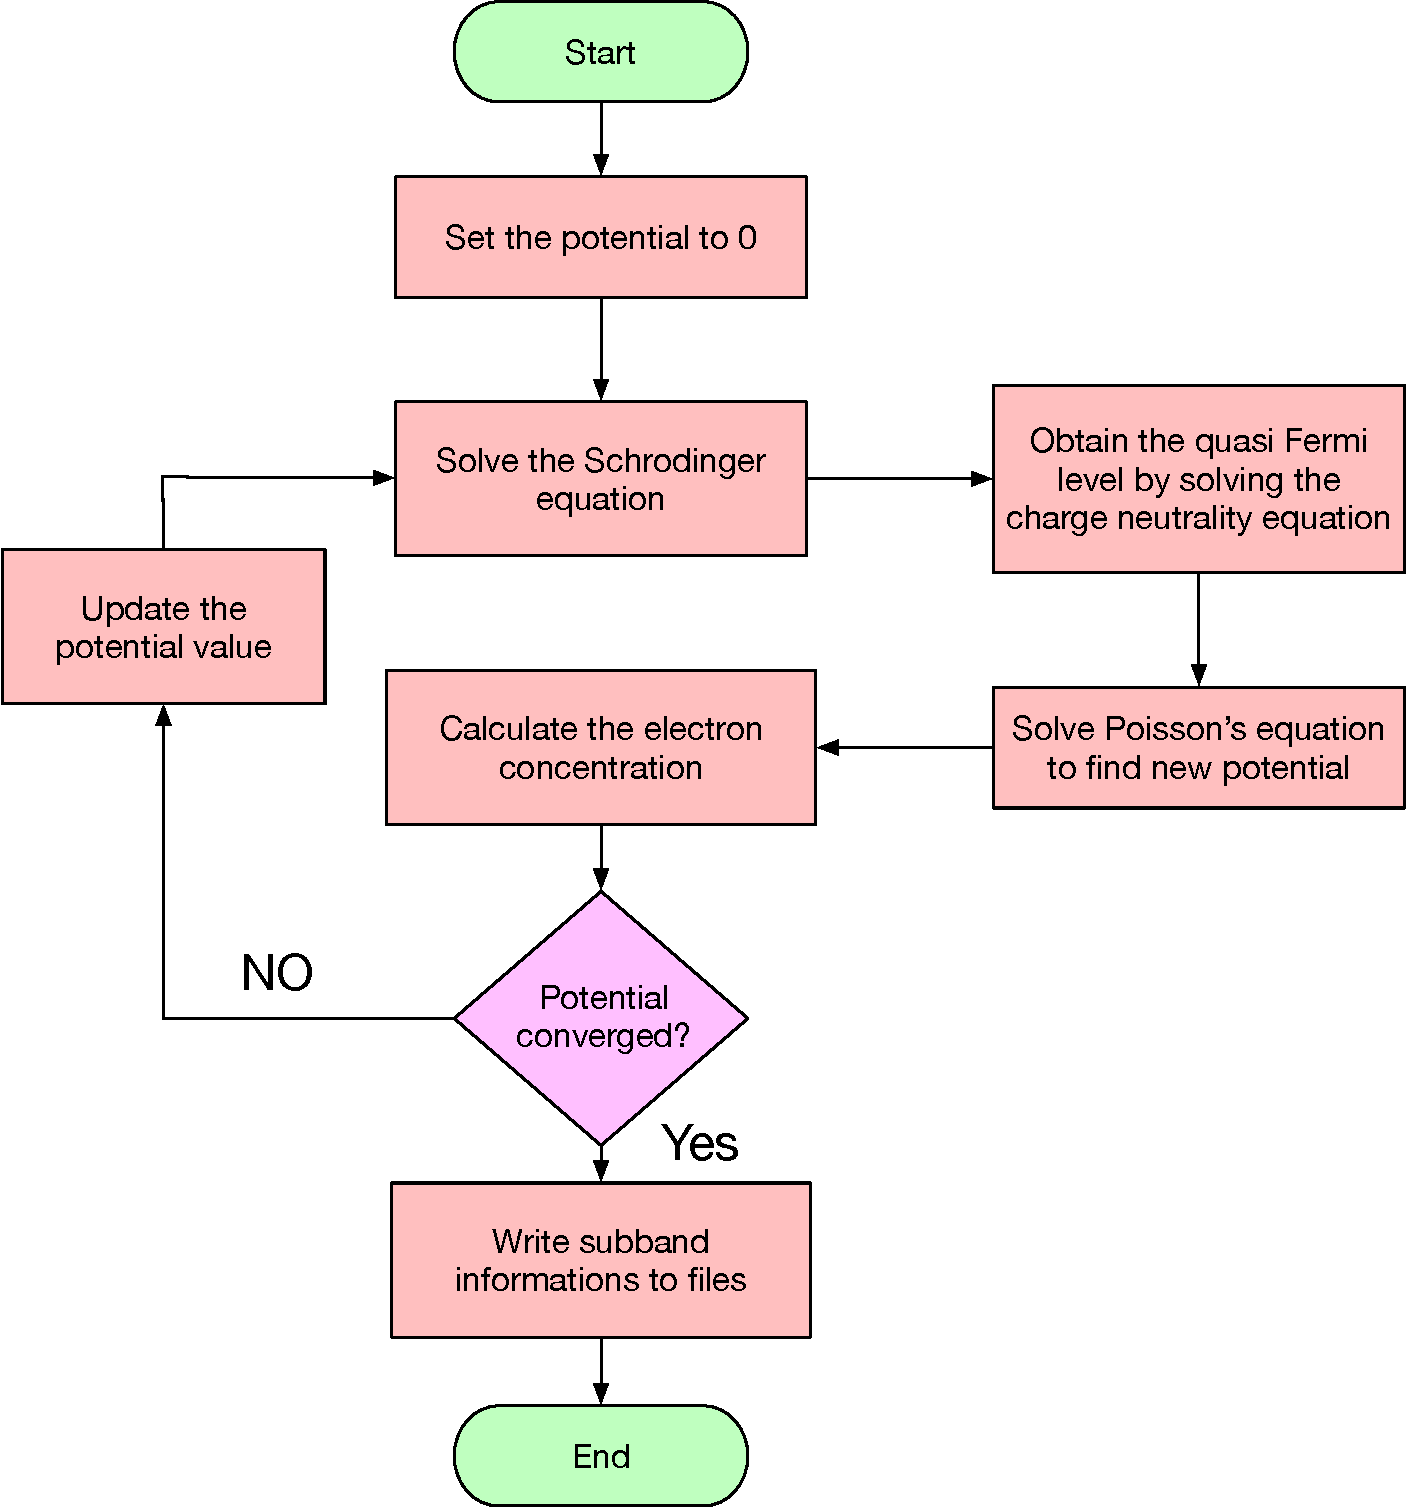
\includegraphics[width=\textwidth]{pictures/ED/SchrodingerPoissonSolver}
  \label{SchrodingerPoissonSolver}
\end{figure}

\section{Electronic Distribution in Nanowires} \label{sec:spectra}

The electronic band structure and the electronic density of cylindrical and
hexagonal GaAs/AlGaAs core-shell nanowire are calculated self-consistently by
solving Poisson and Schr{\"o}dinger equations
\cite{wong2011nanoscale,bertoni2011electron} using $\bf{nextnano^3}$ simulation
packages \cite{birner2007nextnano}, which is a commercial computer aid software
with better physical method for the calculation of the quantum mechanical
properties of an arbitrary combination of geometries and materials.

\subsection{Cylindrical Core-Shell Nanowire}

The cylindrical core-shell nanowire has been investigated with a radius of 20nm
GaAs core and 15nm AlGaAs shell. An additional Si-doped AlGaAs layer with a
0.33 mole fraction is placed between the core and shell. The thickness of this
layers is 5 nm. The left part of Fig.~\ref{CylindricalCSNW} shows the electron
density distribution in 3D view. A free-electron gas is formed in the GaAs core
and at the inner heterointerface with a small fluctuation of density along the
interface. There is a very small amount of electron gas distributed at the
center of the core. Further simulation with different doping density $\rho_D$
shows similar distribution of the electron gas but very small variation of the
magnitude of the intensity. On the right part of Fig.~\ref{CylindricalCSNW},
the black line represents the conduction and valence band bending and the blue
line shows the electron density along the vertical cut of this cylindrical
CSNW.

\begin{figure}
  \caption{(left) Electron charge distribution in 3D illustration. (right) Conduction and valence band bending (black lines) and electron density distribution (blue line) for cylindrical core-shell nanowire. The inset shows the data captured from a vertical slice of the simulated structure.}
  \centering
  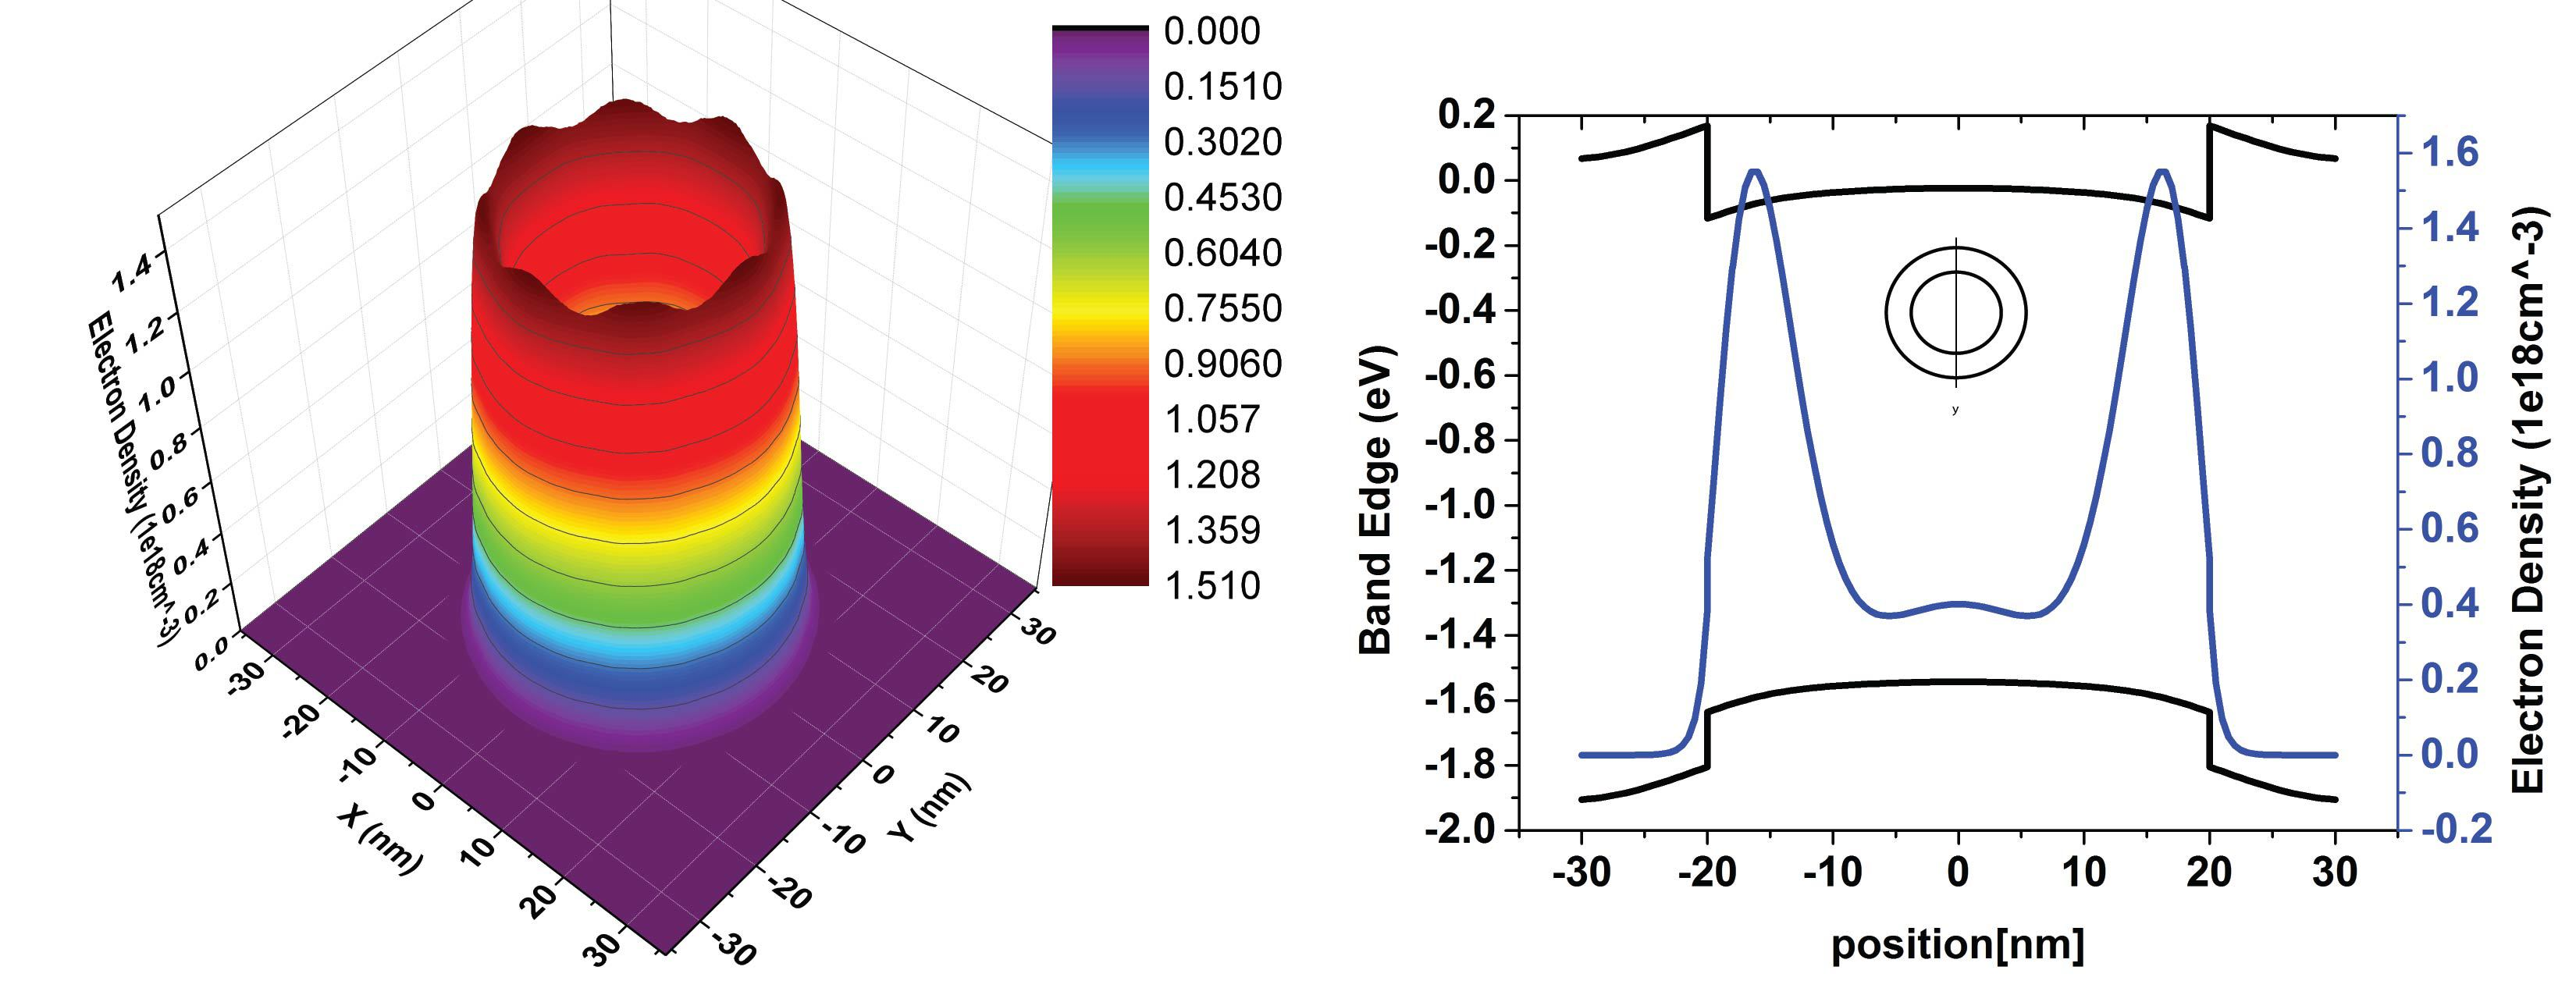
\includegraphics[width=\textwidth]{pictures/ED/CylindricalCSNW}
  \label{CylindricalCSNW}
\end{figure}

\subsection{Hexagonal Core-shell Nanowire} \label{sec:indv_lines}

Due to the hetero-interface between the core and shell and the piezoelectric
force at the corners, the electronic states distribution inside of the
hexagonal core-shell nanowire is not always three-dimensional case or
two-dimensional like in cylindrical NWs. Lower-dimensional electron gas arises
with increased doping density. A delta-doped hexagonal CSNW heterostructure has
been simulated. The radius of GaAs core and AlGaAs shell is 43.3 nm and 45 nm,
respectively, with a 17.3 nm AlGaAs spacer in between. The thickness of
Si-doped AlGaAs is 1.6 nm with a 0.33 mole fraction of AlGaAs. This Si-doped
AlGaAs layer is used to populate a (triangular) quantum well at the
heterointerfaces. Such a well can also be produced by sandwiching a GaAs layer
radially between two wider bandgap materials. 

The left part of Fig.~\ref{3DCharge}, \ref{2DCharge} and \ref{1DCharge} shows
the spatial distribution of the free-electron gas for the three values of the
doping density indicated as (Fig.~\ref{3DCharge}) $\rho_D = 9.2 \times 10^{18}
cm^{-3}$, (Fig.~\ref{2DCharge}) $\rho_D = 9.6 \times 10^{18} cm^{-3}$,
(Fig.~\ref{3DCharge}) $\rho_D = 1.5 \times 10^{19} cm^{-3}$. On the right part,
the electronic band structure (blue line) and the electronic density (red line)
of hexagonal GaAs/AlGaAs core-shell nanowire are depicted for vertical slice
(top, right) or horizontal slice (bottom, right).

At the lowest doping, shown in Fig.~\ref{3DCharge}, the charge is distributed
deep into the core. The distribution is only slightly modulated (right panels)
crossing the core along either the y cross section or x cross section, and
slightly depleted in the center of the core.

\begin{figure}
  \caption{(left) Three dimensional electron charge distribution in 3D illustration. (right) Conduction and valence band bending (blue lines) and electron density distribution (red line) for hexagonal core-shell nanowire with a low doping density. The inset shows the data captured from a (top) vertical or (bottom) horizontal slice of the simulated structure.}
  \centering
  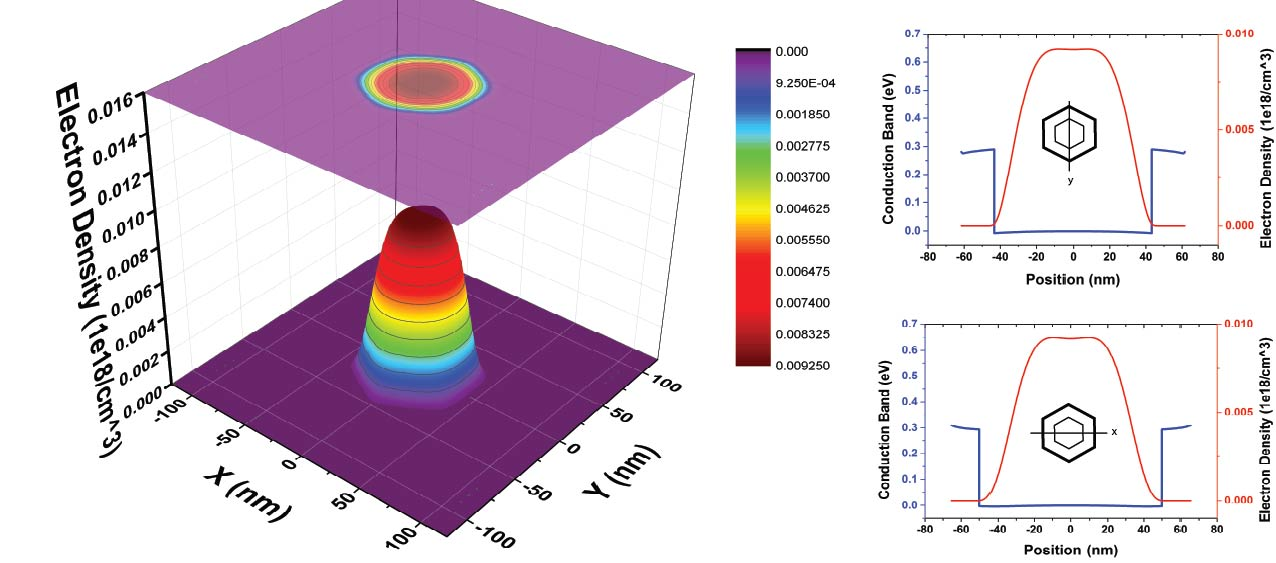
\includegraphics[width=\textwidth]{pictures/ED/3DCharge}
  \label{3DCharge}
\end{figure}

As the doping is increased in Fig.~\ref{2DCharge}, the charge depletion in the
center is more pronounced, and the charge moves toward the heterojunction
interface, leaving this "volcano" like charge distribution in the left part of
Fig.~\ref{2DCharge}. The two-dimensional electron gases (2DEG) are formed at the
heterointerface of GaAs core and AlGaAs shell.

\begin{figure}
  \caption{(left) Two dimensional electron charge distribution in 3D illustration. (right) Conduction and valence band bending (blue lines) and electron density distribution (red line) for hexagonal core-shell nanowire with a moderate doping density. The inset shows the data captured from a (top) vertical or (bottom) horizontal slice of the simulated structure.}
  \centering
  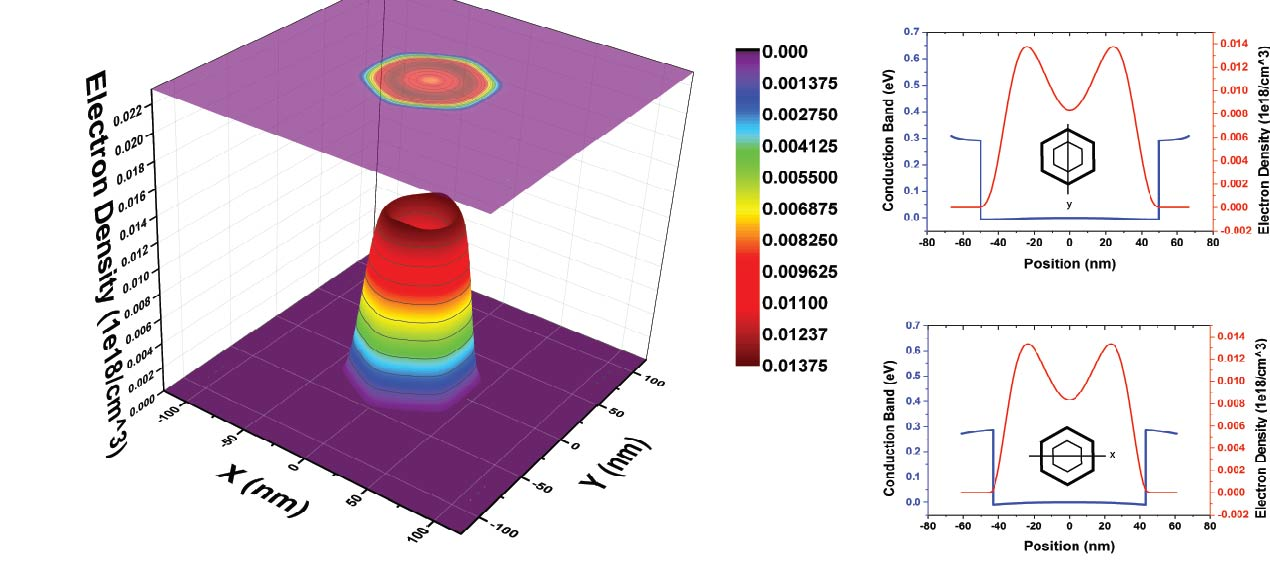
\includegraphics[width=\textwidth]{pictures/ED/2DCharge}
  \label{2DCharge}
\end{figure}

As the doping is further increased in Fig.~\ref{1DCharge}, the shell 2DEG form
at the six (6) core-shell hetero-interface facets, with six (6) pillars of
one-dimensional electron gas (1DEG) forming at the 6 vortices. In addition, as
shown in the right part of the Fig.~\ref{3DCharge}, \ref{2DCharge} and
\ref{1DCharge}, the electronic density of Fig.~\ref{1DCharge} is around two
orders of magnitude higher than 2DEG and bulk counterparts. The results also
matched the other groups' simulation results very well~\cite{Wong:2011tn,
Bertoni:2011hn}.


\begin{figure}
  \caption{(left) One dimensional electron charge distribution in 3D illustration. (right) Conduction and valence band bending (blue lines) and electron density distribution (red line) for hexagonal core-shell nanowire with a high doping density. The inset shows the data captured from a (top) vertical or (bottom) horizontal slice of the simulated structure.}
  \centering
  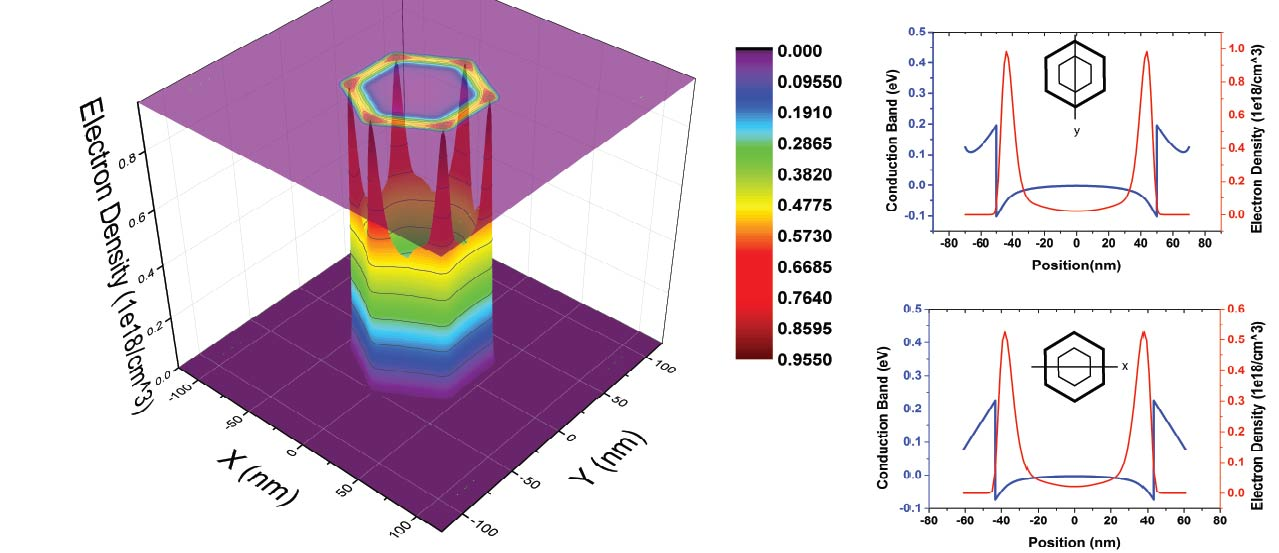
\includegraphics[width=\textwidth]{pictures/ED/1DCharge}
  \label{1DCharge}
\end{figure}


\section{Conclusions} \label{sec:conclusions}

In this chapter, the finite-element-method implemented self-consistent
Shr{\"o}dinger-Poisson solver has been discussed. In addition, a cylindrical
and hexagonal core-shell nanowire structure has been simulated and compared
with different doping density. The simulated results show unique electron
density distribution in hexagonal CSNW with large doping density. This unique
distribution of electrons has also been verified experimentally by electron
holographic tomography~\cite{Wolf:2011if} 
